

%% CAP High School Prize Examination
%%----------------------------------------


%% this section contains 40 problems


%% CAP Exam 2015
%%----------------------------------------


%% CAP Exam 2013
%%----------------------------------------
\element{cap}{ %% cap-C1
\begin{question}{CAP-A-2013-q13}
    You put two identical ice cubes on plates of different materials. 
    One cube is put on an aluminum plate,
        and the other on a glass plate. 
    Both plates have been in the room for a long time prior to the experiment. 
    You notice that the ice melts faster on the metal plate. 
    Why?
    \begin{choices}
        \wrongchoice{The ice is in thermal equilibrium with the plastic plate, but not with the metal plate.}
      \correctchoice{The metal plate conducts heat to the ice more rapidly than the plastic plate.}
        \wrongchoice{The metal plate holds more heat than the plastic plate.}
        \wrongchoice{The metal plate was warmer than the plastic plate initially.}
    \end{choices}
\end{question}
}


%% CAP Exam 2012
%%----------------------------------------
\element{cap}{ %% cap-C1
\begin{question}{CAP-A-2012-q07}
    The Earth is constantly receiving energy from the Sun.
    To stay at approximately the same temperature,
        the Earth loses energy by:
    \begin{choices}
        \wrongchoice{Conduction}
      \correctchoice{Radiation}
        \wrongchoice{Convection}
        \wrongchoice{Evaporation}
        \wrongchoice{The Earth does not lose energy, this is why we have global warming.}
    \end{choices}
\end{question}
}

\element{cap}{ %% cap-C1
\begin{question}{CAP-A-2012-q19}
    An aluminum plate and a glass plate are left in a room for a long time. 
    Putting one ice cube on each plate,
        you notice that the ice melts faster on the aluminum plate. 
    Why?
    \begin{choices}
        \wrongchoice{The ice is in thermal equilibrium with the glass plate, but not with the aluminum plate.}
      \correctchoice{Aluminum conducts heat to the ice more rapidly than glass.}
        \wrongchoice{The aluminum plate holds more heat.}
        \wrongchoice{The aluminum plate is warmer.}
    \end{choices}
\end{question}
}


%% CAP Exam 2011
%%----------------------------------------
\element{cap}{ %% cap-C1
\begin{question}{CAP-A-2011-q15}
    Objects $A$ and $B$, isolated from the environment,
        are initially separated from each other and are then placed in thermal contact. 
    Their initial temperatures are $T_A=\SI{0}{\degreeCelsius}$ and $T_B=\SI{100}{\degreeCelsius}$. 
    The heat capacity of $B$ is twice the one of $A$. 
    \begin{center}
    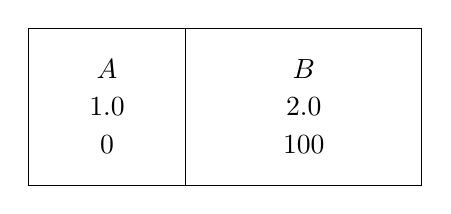
\begin{tikzpicture}
        %% Block A
        \draw (0,0) rectangle (2,2);
        %% label A
        \node[anchor=center] (A) at (1,1) {\SI{1.0}{\kilo\gram}};
        \node[anchor=south] at (A.north) {$A$};
        \node[anchor=north] at (A.south) {\SI{0}{\degreeCelsius}};
        %% Block B
        \draw (2,0) rectangle (5,2);
        %% label B
        \node[anchor=center] (B) at (3.5,1) {\SI{2.0}{\kilo\gram}};
        \node[anchor=south] at (B.north) {$B$};
        \node[anchor=north] at (B.south) {\SI{100}{\degreeCelsius}};
    \end{tikzpicture}
    \end{center}
    After a certain time, the system reaches equilibrium. 
    The final temperatures are:
    \begin{choices}
        \wrongchoice{$T_A = T_B = \SI{50}{\degreeCelsius}$}
      \correctchoice{$T_A = T_B > \SI{50}{\degreeCelsius}$}
        \wrongchoice{$T_A = T_B < \SI{50}{\degreeCelsius}$}
        \wrongchoice{$T_A > T_B > \SI{50}{\degreeCelsius}$}
        \wrongchoice{$T_A > \SI{50}{\degreeCelsius} > T_B$}
    \end{choices}
\end{question}
}

\element{cap}{ %% cap-C1
\begin{question}{CAP-A-2011-q19}
    This graph shows the average temperature inside a room. 
    \begin{center}
    \begin{tikzpicture}
        \begin{axis}[
            axis y line=left, 
            axis x line=bottom, 
            axis line style={->},
            xlabel={time},
            xtick={4,8},
            xticklabels={$t_1$,$t_2$},
            x label style={
                at={(current axis.right of origin)},
                anchor=north east,
            },
            ylabel={temperature},
            ytick=\empty,
            xmin=0,xmax=13,
            ymin=0,ymax=11,
            grid=major,
            width=0.8\columnwidth,
            height=0.5\columnwidth,
        ]
        \addplot[line width=1pt] plot coordinates { (0,2) (4,2) };
        \draw (axis cs:4,2) to[out=70,in=180] (axis cs:8,7);
        \addplot[line width=1pt] plot coordinates { (8,7) (12,7) };
        \node[anchor=center] at (axis cs:2,9) {I};
        \node[anchor=center] at (axis cs:6,9) {II};
        \node[anchor=center] at (axis cs:10,9) {III};
        \end{axis}
    \end{tikzpicture}
    \end{center}
    At time $t_1$ the heater is turned on. 
    We want to compare the power input to the room ($P_{\text{in}}$) and the power output from the room ($P_{\text{out}}$).
    For which region(s) on the graph is $P_{\text{in}} \neq P_{\text{out}}$?
    \begin{choices}
        \wrongchoice{Only region I}
      \correctchoice{Only region II}
        \wrongchoice{Only region III}
        \wrongchoice{Only regions I \& III}
        \wrongchoice{Regions I, II \& III}
    \end{choices}
\end{question}
}


%% CAP Exam 2009
%%----------------------------------------
\element{cap}{ %% cap-C1
\begin{question}{CAP-A-2009-q03}
    We know that a person emits about \SI{500}{\watt} of radiation.
    We also know that a person sitting still uses about \SI{100}{\watt} of chemical energy.
    Where is the rest of the energy mainly coming from?
    \begin{choices}
        \wrongchoice{Heat conducted from the air into our body.}
        \wrongchoice{Convection of the heat.}
      \correctchoice{Radiation from objects around us.}
        \wrongchoice{The energy, emitted by the body does not have to have a source.}
        \wrongchoice{Burning fat that we have accumulates previously.}
    \end{choices}
\end{question}
}

\element{cap}{ %% cap-C1
\begin{question}{CAP-A-2009-q06}
    Objects $A$ and $B$ that are initially separated from each other and well isolated from their surroundings are then brought into thermal contact.
    Initially $T_A = \SI{0}{\degreeCelsius}$ and $T_B = \SI{100}{\degreeCelsius}$.
    \begin{center}
    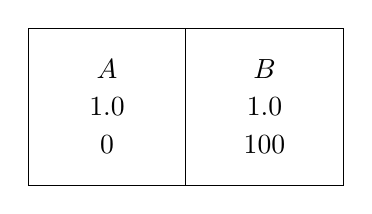
\begin{tikzpicture}
        %% Block A
        \draw (0,0) rectangle (2,2);
        %% label A
        \node[anchor=center] (A) at (1,1) {\SI{1.0}{\kilo\gram}};
        \node[anchor=south] at (A.north) {$A$};
        \node[anchor=north] at (A.south) {\SI{0}{\degreeCelsius}};
        %% Block B
        \draw (2,0) rectangle (4,2);
        %% label B
        \node[anchor=center] (B) at (3,1) {\SI{1.0}{\kilo\gram}};
        \node[anchor=south] at (B.north) {$B$};
        \node[anchor=north] at (B.south) {\SI{100}{\degreeCelsius}};
    \end{tikzpicture}
    \end{center}
    The specific heat of $A$ is less than the specific heat of $B$.
    After some time,
        the system comes to an equilibrium state.
    Their final temperatures are:
    \begin{choices}
      \correctchoice{$T_A = T_B > \SI{3.9}{\degreeCelsius}$}
        \wrongchoice{$T_A > T_B > \SI{3.9}{\degreeCelsius}$}
        \wrongchoice{$T_A = T_B < \SI{3.9}{\degreeCelsius}$}
        \wrongchoice{$T_B > T_A > \SI{3.9}{\degreeCelsius}$}
        \wrongchoice{$T_A = T_B = \SI{3.9}{\degreeCelsius}$}
    \end{choices}
\end{question}
}


\endinput


